\documentclass{article}
\usepackage{amsmath}
\usepackage{array}
\usepackage{siunitx}  
\usepackage{tikz}
\usepackage{tkz-euclide}
\usepackage[numbib]{tocbibind}
\usepackage{hyperref}
\usepackage{float}
\begin{document}

\title{Low SNR FreeDV Mode}
\author{David Rowe VK5DGR}
\maketitle

\section{Introduction}

After 10 years development and on air experience with various FreeDV waveforms, we would like to develop a new waveform that outperforms and replaces a variety of existing modes such as 700C/D/E and 1600.  Requirements include \cite{freedv-020}:
\begin{enumerate}
\item Better performance than SSB at 0dB SNR on MPP and MPD channels.
\item A single mode that can handle MPP, MPD, GEO (e.g. QO-100), and replace several existing FreeDV modes, simplifying the end user experience.
\item For compliance with Export Control regulations, the minimum speech codec bit rate is 700 bit/s.
\item Use of legacy analog HF radio sets with a RF bandwidth of around 2000 Hz.
\item Compliant with the 300 baud per carrier limit set by the United States FCC, which implies a parallel tone or OFDM modem. 
\end{enumerate}
It is acceptable for performance to gradually decrease as the multipath channel quality declines, but we would like the decline to be gradual, e.g. a few dB more power for operation on MPD versus MPP.

This document explores ways we can improve the existing OFDM modem waveforms in order to meet these requirements.

\clearpage

\subsection{Glossary}

\begin{table}[h]
\centering
\begin{tabular}{l p{8cm} }
 \hline
 Acronym & Explanation \\
 \hline
 AWGN & Additive White Gaussian Noise - a communications channel with flat frequency response and additive noise \\
 CP & Cyclic Prefix \\
 FEC & Forward Error Correction \\
 ISI & Inter Symbol Interference \\
 LEO & Low earth orbit satellite channel, AWGN with large freq offset and Doppler shift (high rate of change of freq offset) \\
 GEO & Geosynchronous satellite channel, AWGN but high phase noise and large freq offset \\
 OTA & Over The Air \\
 PTT & Push To Talk - voice communications where only one person is transmitting at any one time.  Common in two way radio but not mobile telephones  \\
 MPP & Multipath Poor channel, 1 Hz Doppler spread, 2ms delay spread, typical for US and Australian interstate propogation \\
 MPD & Multipath Disturbed channel, 2 Hz Doppler spread, 4ms delay spread, typical for UK Winter NVIS propogation \\
 \hline
\end{tabular}
\caption{Glossary of Acronyms}
\end{table}

\begin{table}[h]
\centering
\begin{tabular}{l m{6cm} l}
 \hline
 Symbol & Explanation & Units \\
 \hline
 $B$ & Noise or signal bandwidth & Hz \\
 $B_d$ & Doppler spreading bandwidth for HF channel model & Hz \\
 $D$ & Algorithmic delay, how much speech we need to buffer before processing starts & seconds \\
 $E_b/N_0$ & Energy per bit on spectral noise density & dimensionless, dB\footnote{1} \\
 $N_s$ & Number of symbols in a \emph{modem frame}, pilot insertion rate  \\
 $R_b$ & Bit rate & Bits/second \\
 $R_s$ & Symbol rate & symbols/second \\
 $T_s$ & Symbol period & seconds \\
 $SNR$ & Signal to Noise Ratio & dB \\
 $S$ & Signal Power & Watts \\
 $N$ & Noise Power & Watts \\
 $N_c$ & Number of carriers in an OFDM waveform \\
 \hline
\end{tabular}
\caption{Glossary of Symbols}
\end{table}

\footnotetext[1]{Can be expressed as a linear ratio $E_b/N_0$ or $10log_{10}(E_b/N_0)$ dB}

\clearpage

\section{Modem and Channel Models}

In this section we will develop theoretical models to help us explore performance limits.

\subsection{SNR and Bandwidth Limits}

For practical PTT voice systems algorithmic delay is limited to a few 100ms, which limits the FEC codeword size and hence the performance of the code.  For PSK channels a threshold $E_b/N_0=2 \, \si{dB}$ and a code rate $R=0.5$ is typical, where $E_b/N_0$ is the energy per payload data bit (coded $E_b/N_0$).  The lowest (threshold) SNR for a viable voice link is given by:
\begin{equation}
\label{eq:snr}
\begin{split}
\frac{S}{N} &= \frac{E_bR_b}{N_0B} \\
SNR &= 10log_{10}\left(\frac{E_b}{N_0}\right) + 10log_{10}\left(\frac{R_b}{B}\right) \quad [\si{dB}]
\end{split}
\end{equation}
where $R_b$ is the payload data bit rate, and $B$ is the bandwidth in which we measure SNR.  Given $Rb=700$ and $B=3000$ we have:
\begin{equation}
\begin{split}
SNR &= 2 + 10log_{10}(700/3000) \\
    &= -4.3 \, \si{dB}
\end{split}
\end{equation}
This is ideal performance for an AWGN channel.  In practice we must allocate some power to symbols used for synchronisation, such as pilot symbols used for frequency and phase estimation, or unique word bits used for frame synchronisation.  Synchronisation algorithms often struggle at low SNRs, introducing additional "implementation" losses.

Performance on multipath channels is significantly worse, in our use cases typically 5 dB.  On these channels, we may allocate some carrier power to deal with intersymbol interference (for example a cyclic prefix in OFDM modems).

A more complete model is:
\begin{equation}
\label{eq:snr_all}
SNR = 10log_{10}\left(\frac{E_b}{N_0}\right) + 10log_{10}\left(\frac{R_b}{B}\right) + L_p + L_{il} + L_{cp}
\end{equation}
where $L_p$ is the loss from power allocated to pilot symbols, $L_{il}$ is the real world implementation loss, and $L_{cp}$ is the loss in SNR due to the power allocated to the cyclic prefix.

To combat intersymbol interference and Doppler Spread on HF multipath channels, it is convenient to use parallel tone or OFDM modems. The signal is divided into $N_c$ carriers, each carrying $R_b/N_c$ bits/s.  Due to the spectral efficiency of OFDM, the same bit rate, symbol rate, and occupied bandwidth is required for any $N_c$.  For example:
\begin{enumerate}
\item A QPSK signal of $R_s=1000$ symbols/s and $R_b=2R_s=2000$ bits/s occupies $B=1000$ Hz (central lobe).
\item An OFDM signal of $N_c=20$ carriers each at $R_s=50$ symbol/s gives us a total $R_b=2N_cR_s=2000$ bits/s and occupies a RF bandwidth of $B=N_cR_s=1000$ Hz.
\end{enumerate}
This simple relationship between per-carrier and total $R_s$ allows us to use them interchangeably for some calculations.
 
FreeDV signals are typically transmitted over the air using analog HF radios.  We assume a RF bandwidth of 2000 Hz is available, which allows a maximum of 4000 bit/s using QPSK.  In practice the payload data rate is much less, due to various overheads that we will discuss below.

\subsection{Pilot Symbol Overhead}

\begin{figure}[h]
\caption{Modem Frame with $N_s=8$, the pilot of the next modem frame is also shown.}
\vspace{5mm}
\label{fig:modem_frame}
\centering
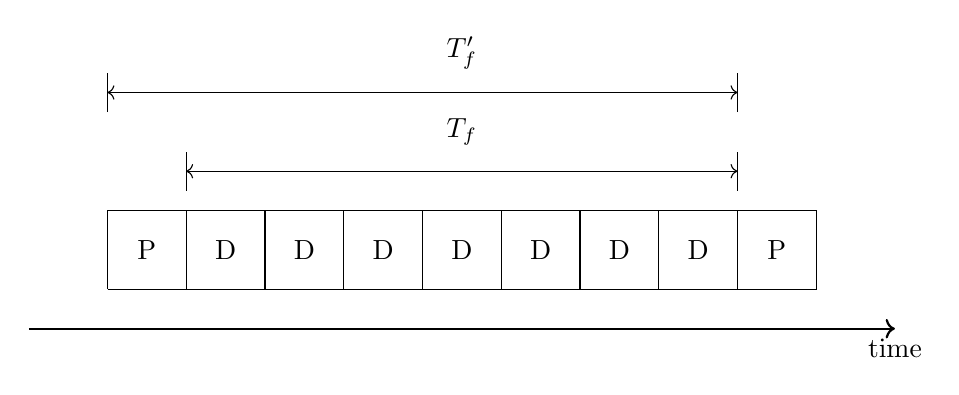
\begin{tikzpicture}
\draw[thick,->] (0,0.5) -- (11,0.5) node [below]{time};
\draw (1,1) -- (10,1) -- (10,2) -- (1,2) -- (1,1);
\draw (2,1) -- (2,2); \draw (3,2) -- (3,1); \draw (4,2) -- (4,1);
\draw (5,1) -- (5,2); \draw (6,2) -- (6,1); \draw (7,2) -- (7,1);
\draw (8,2) -- (8,1); \draw (9,2) -- (9,1);
\node[align=center] at (1.5,1.5) {P}; \node[align=center] at (9.5,1.5) {P};
\foreach \x in {2,3,4,5,6,7,8}
  \node[align=center] at (\x.5,1.5) {D};
\draw (2,2.25) -- (2,2.75); \draw (9,2.25) -- (9,2.75); 
\draw [<->] (2,2.5) -- (9,2.5);
\node[align=center] at (5.5,3) {$T_f$};
\draw (1,3.25) -- (1,3.75); \draw (9,3.25) -- (9,3.75); 
\draw [<->] (1,3.5) -- (9,3.5);
\node[align=center] at (5.5,4) {$T^\prime_f$};
\end{tikzpicture}
\end{figure}

In this section we explore the effect of inserting pilot symbols on the threshold SNR (\ref{eq:snr}). Consider a sequence of $N_s-1$ PSK data symbols that carry the modulated FEC codeword bits (e.g. data and parity bits) over the channel. We denote this sequence a modem \emph{modem frame}. The frame of $N_s-1$ symbols has a period of $T_f=(N_s-1)T_s$ seconds, where $T_s$ is the period of each symbol.  We wish to insert a single pilot symbol after the data symbols, creating a new frame $N_s$ symbols long, with period $T^\prime_f=N_sT_s$.  To maintain the same payload data rate:
\begin{equation}
\begin{split}
T_f &= T^\prime_f \\
(N_s-1)T_s &= N_sT_s \\
R^\prime_s &= R_s\frac{N_s}{N_s-1}
\end{split}
\end{equation}
where the symbol rate $R_s=1/T_s$.  Expressing $S/N$ (\ref{eq:snr}) in terms of $E_s$ and $R_s$:
\begin{equation}
\label{eq_snr_s}
\begin{split}
\frac{S}{N} &= \frac{E_sR_s}{N_0B} \\
\frac{S}{N}^\prime &= \frac{E_sR^\prime_s}{N_0B} \\
                   &= \frac{E_sR_sN_s}{N_0B(N_s-1)} \\
\frac{S^\prime/N}{S/N} &= \frac{N_s}{N_s-1}
\end{split}
\end{equation}
Thus when we insert pilots, the threshold $S/N$ increases by a factor of $N_s/(N_s-1)$. Expressed in $\si{dB}$:
\begin{equation}
\begin{split}
10log_{10}\left(\frac{S^\prime}{N}\right) &= 10log_{10}\left(\frac{S}{N}\right) + 10log_{10}\left(\frac{N_s}{N_s-1}\right) \\
SNR^\prime &= SNR + 10log_{10}\left(\frac{N_s}{N_s-1}\right) \\
SNR^\prime &= SNR + L_p  \quad [\si{dB}]
\end{split}
\end{equation}
where $L_p$ can be considered the pilot symbol \emph{loss} - the SNR degradation from the ideal performance (\ref{eq:snr}) due to the insertion of pilot symbols. For example FreeDV 700D uses a pilot insertion rate of $N_s=8$ results in $L_p=10log_{10}(8/7)=0.58 \, \si{dB}$, thus we need 0.58 dB more SNR to achieve the threshold SNR for the voice link.   For this example let $Rs$ be the total symbol rate over all $N_c$ carriers. To maintain $Rs=700$ data symbols/second over the channel, we require $R^\prime_s = (700)8/7 =800$ symbols/second which introduces a 100 Hz bandwidth overhead.

\subsection{Cyclic Prefix Overhead}

\begin{figure}[h]
\caption{Construction of composite symbol with a Cyclic Prefix CP pre-pended to a shortened data symbol $D^\prime$.}
\vspace{5mm}
\label{fig:composite_symbol}
\centering
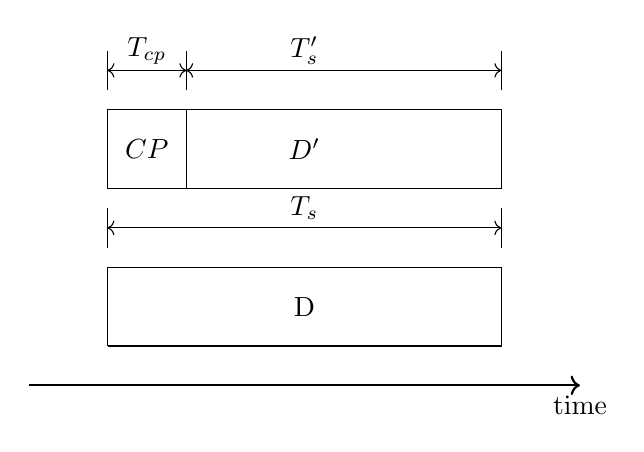
\begin{tikzpicture}
\draw[thick,->] (0,0.5) -- (7,0.5) node [below]{time};

\draw (1,1) -- (6,1) -- (6,2) -- (1,2) -- (1,1);
\node[align=center] at (3.5,1.5) {D};

\draw (1,2.25) -- (1,2.75); \draw (6,2.25) -- (6,2.75); 
\draw [<->] (1,2.5) -- (6,2.5);
\node[align=center] at (3.5,2.75) {$T_s$};

\draw (1,3) -- (6,3) -- (6,4) -- (1,4) -- (1,3);
\draw (2,3) -- (2,4);
\node[align=center] at (3.5,3.5) {$D^\prime$};
\node[align=center] at (1.5,3.5) {$CP$};

\draw (1,4.25) -- (1,4.75); \draw (2,4.25) -- (2,4.75); \draw (6,4.25) -- (6,4.75); 
\draw [<->] (1,4.5) -- (2,4.5);
\node[align=center] at (1.5,4.75) {$T_{cp}$};
\draw [<->] (2,4.5) -- (6,4.5);
\node[align=center] at (3.5,4.75) {$T^\prime_s$};

\end{tikzpicture}
\end{figure}

Now we consider the SNR overhead for the Cycle Prefix (CP) used in OFDM modems to cope with delay spread on multipath channels.  To achieve our payload data rate (e.g. 700 bits/s), we FEC encode and map the bits to PSK symbols $D$, and distribute the symbols across $N_c$ parallel carriers.  The transmitter power is spread equally across all carriers.

We send symbols $D$ across the channel at a constant symbol rate $R_s$, or one symbol every $T=T_s$ seconds.  To cope with delay spread, we construct a composite symbol by pre-pending a Cyclic Prefix (CP) $T_{cp}$ seconds in duration to a new symbol $D^\prime$ of $T^\prime_s$ seconds in duration.  $D$ and $D^\prime$ contain the same PSK symbol, and convey the same information over the channel. The new composite symbol is now $T^\prime = T_{cp}+T^\prime_s$ seconds long.  The CP contains no additional information, it is just a cyclic extension of the single symbol $D^\prime$. Thus we still send one symbol of data over the channel every $T^\prime$ seconds.  To maintain the payload data rate over the channel, we must send the new composite symbol at the same rate as the original symbol:
\begin{equation}
\begin{split}
T &= T^\prime \\
T_s &= T_{cp} + T^\prime_s \\
R^\prime_s &= \frac{R_s}{1 - T_{cp}/T_s}
\end{split}
\end{equation}
It can be observed that $R^\prime_s > R_s$, to account for the portion of the composite symbol allocated to the CP.  For example with $R_s=50$, $T_s=0.02$, $T_{cp}=0.002$, $R^\prime_s=50/(1-0.002/0.02)=55.56$ symbols/second.  Thus additional bandwidth is required to send the composite symbol including the cyclic prefix.

The increase in symbol rate does not directly affect BER performance if $E_s/N_0$ remains the same. For example if $Rs^\prime=2R_s$ we could send the symbol across the channel in $T_s/2$ seconds at power $2S$, followed by $T_s/2$ seconds of silence.  The energy per symbol $E_s$ and BER would remain the same.

For the composite symbol, the transmitter power $S^\prime$ is spread between the CP and $D^\prime$.  Given a constant power $S^\prime$, the energy for the symbol $D^\prime$ is given by:
\begin{equation}
\begin{split}
E^\prime_s &= \frac{S^\prime}{R^\prime_s}  \\
           &= \frac{S^\prime}{R_s}(1 - T_{cp}/T_s)
\end{split}
\end{equation}
For the link BER to be maintained the energy per symbol must be unchanged, i.e. $E^\prime_s=E_s$:
\begin{equation}
\begin{split}
E_s           &= \frac{S^\prime}{R_s}(1 - T_{cp}/T_s) \\
\frac{S}{R_s} &= \frac{S^\prime}{R_s}(1 - T_{cp}/T_s) \\
\frac{S}{N} &= \frac{S^\prime}{N}(1 - T_{cp}/T_s) \\
\frac{S^\prime}{N} &= \frac{S}{N}\left(\frac{1}{1 - T_{cp}/T_s}\right) \\
SNR^\prime  &= SNR - 10log_{10}(1-T_{cp}/T_s) \\
            &= SNR + L_{cp} \quad [\si{dB}] \\
     L_{cp} &= -10log_{10}(1-T_{cp}/T_s)    
\end{split}
\end{equation}
Thus to close the link with the composite symbol the $S/N$ must be increased by a factor of $1/(1 - {T_s}/T_{cp})$ compared to our ideal modem, to account for the energy allocated to the CP.  For example FreeDV 700E has $T_s=0.02$, $T_{cp}=0.006$, giving $L_{cp}=-10log10(1-0.006/0.02)=1.55 \si{dB}$.

\subsection{Bandwidth}

Using the expressions above, we can estimate the total RF bandwidth of candidate waveforms:
\begin{equation}
B = \frac{R_sN_s}{(N_s-1)(1-T_{cp}/T_s)}
\end{equation}

where $R_s$ is the total symbol rate over the channel.  For example for 700D, $B = 700(8)/((8-1)(1-0.002/0.02))=888.89$ Hz.  In practice 700D has some extra bits allocated for frame synchronisation and auxiliary text, resulting in $B=944$ Hz.

\subsection{Latency}
\label{sec:latency}

Latency is delay experienced by end users when using a speech processing system such as FreeDV. Latency is an important trade off for real time, Push To Talk (PTT) speech communication. Speech compression and FEC tend to work better with latency, but subjective quality tends to decrease whenever there is delay in conversational speech.

The algorithmic delay is defined as the number of seconds $D$ of signal that must be collected in order to start processing. A typical speech codec will collect 20-40ms of speech samples before starting analysis.  However much longer FEC codewords sizes are desirable in order to ride over fades.  For example FEC codeword sizes spanning several seconds are common for HF data modes.  For maximum robustness, interleaving require all bits in the codewords to be received before FEC decoding starts.  The modem may also introduce delay, for example FreeDV 700D has a one frame look ahead for pilot symbols.

Consider a FreeDV mode with algorithmic delay $D$ seconds (Figure \ref{fig:latency})
\begin{enumerate}
\item First we must collect $D$ seconds of speech samples.
\item The speech samples are encoded and a buffer of $D$ seconds of modem samples generated.
\item The modem samples are sent over the radio channel, where they are buffered at the receiver.
\item When a $D$ second buffer of modem samples is collected at the receiver, the modem samples can be decoded to a buffer of output speech samples.
\item The output speech samples are played to a listener.
\end{enumerate}  

Latency is the time from when a speech sample enters the input buffer to when it is played at the receiver. If we assume infinite CPU such that the encode and decode times are zero, and zero propagation delay across the channel, the minimum latency experienced by an end user is twice the algorithmic delay, or $2D$.

\begin{figure}[h]
\caption{Latency of a waveform with algorithmic delay $D$ seconds}
\vspace{5mm}
\label{fig:latency}
\centering
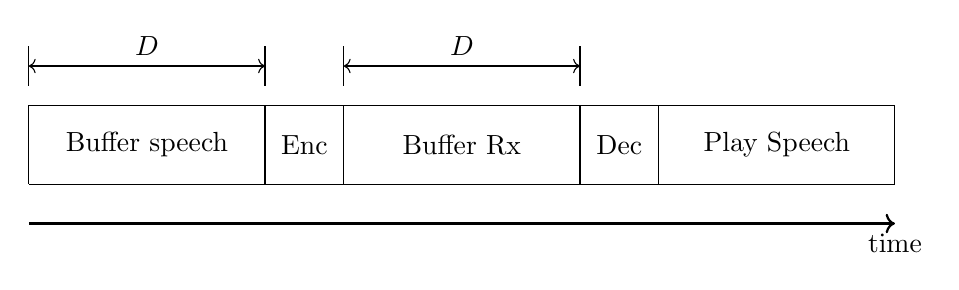
\begin{tikzpicture}
\draw[thick,->] (0,0.5) -- (11,0.5) node [below]{time};

\draw (0,1) -- (3,1) -- (3,2) -- (0,2) -- (0,1);
\node[align=center] at (1.5,1.5) {Buffer speech};

\draw (3,1) -- (4,1) -- (4,2) -- (3,2) -- (3,1);
\node[align=center] at (3.5,1.5) {Enc};

\draw (4,1) -- (7,1) -- (7,2) -- (4,2) -- (4,1);
\node[align=center] at (5.5,1.5) {Buffer Rx};

\draw (7,1) -- (8,1) -- (8,2) -- (7,2) -- (7,1);
\node[align=center] at (7.5,1.5) {Dec};

\draw (8,1) -- (11,1) -- (11,2) -- (8,2) -- (8,1);
\node[align=center] at (9.5,1.5) {Play Speech};

\draw (0,2.25) -- (0,2.75); \draw (3,2.25) -- (3,2.75); 
\draw [<->] (0,2.5) -- (3,2.5);
\node[align=center] at (1.5,2.75) {$D$};

\draw (4,2.25) -- (4,2.75); \draw (7,2.25) -- (7,2.75); 
\draw [<->] (4,2.5) -- (7,2.5);
\node[align=center] at (5.5,2.75) {$D$};

\end{tikzpicture}
\end{figure}

\subsection{Summary of FreeDV modes}

Using the framework developed above and the information in \cite{codec2_waveform_spreadsheet}, we can analyse the existing FreeDV waveforms.

\begin{table}[h]
\label{tab:freedv_wavefoms}
\centering
\begin{tabular}{c c c c c c c c}
 \hline
 Mode & $N_s$ & $R_s$ & $Ts$ & $T^\prime_s$ & $T_{cp}$ & ${L_p}$ (dB) & $L_{cp}$ (dB)  \\
 \hline
 700C & 3 & 75 & 0.013 & 0.013 & 0.000 & 1.77 & 0.00 \\
 700D & 8 & 50 & 0.020 & 0.018 & 0.002 & 0.58 & 0.46 \\
 700E & 4 & 50 & 0.020 & 0.014 & 0.006 & 1.24 & 1.55 \\
 datac4 & 5 & 50 & 0.020 & 0.014 & 0.006 & 0.97 & 1.38 \\
 \hline
\end{tabular}
\caption{Summary of FreeDV waveforms, note the differences in the overheads $L_p$ and $L_{cp}$. $R_s$ and $T_s$ is per-carrier. 700C is a parallel tone modem with no cyclic prefix, the modem frame is comprised of two pilot symbols and 4 data symbols}
\end{table}

TODO: $L_{il}$ estimate using \emph{lin2} modelling below, likely to be greater for 700C/E.  We could also include ${N_c}$, total $R_s$, and SNR estimates.

\subsection{HF Channel Model}

A common two path HF channel model \cite{itu1487} is given by:
\begin{equation}
y(t) = x(t)G_1(t) + x(t-d)G_2(t)
\end{equation}
where $G_1$ and $G_2$ are two time varying, complex, Gaussian filtered random variables with \emph{Doppler Spread} bandwidth $B_d$ Hz, $d$ is the path delay in seconds. Other models with varying delay, number of paths, and fixed frequency offset components are also possible, for example Appendix B of \cite{etsi201}.

As $B_d<< R_s$ we assume $G_1$ and $G_2$ are complex constants for the duration of a single symbol. Expressed in discrete time for the current symbol:
\begin{equation}
\label{eq:hf_model_time}
y(n) = x(n)G_1 + x(n-dF_s)G_2
\end{equation}
where $F_s$ is the sample rate in $\si{Hz}$.  Taking the z-transform:
\begin{equation}
\label{eq:hf_model_freq}
\begin{split}
Y(z) &= X(z)G_1+X(z)z^{-dF_s}G_2 \\
\frac{Y(z)}{X(z)} &= G_1+z^{-dF_s}G_2 \\
H(z) &= G_1+z^{-dF_s}G_2 \\
H(e^{j \omega}) &= G_1+e^{-j \omega d F_s}G_2
\end{split}
\end{equation}

Lets examine the effects of intersymbol interference due to the delay spread.  Consider the transmitter sample $x(0)$ where we transition from one PSK phase $\phi_1$ to the next $\phi_2$.  Near the transition we can define $x(n)$ in terms of a step function $s(n)$:
\begin{equation}
\begin{split}
x(n) &=
	\begin{cases}
      e^{j (\omega n + \phi_1)}, & n < 0 \\
      e^{j (\omega n + \phi_2)}, & n \ge 0
	\end{cases} \\
	&= s(n)e^{j (\omega n + \phi_2)} + (1-s(n))e^{j (\omega n + \phi_1)}  \\
s(n) &=
	\begin{cases}
      0, & n < 0 \\
      1, & n \ge 0
	\end{cases}
\end{split}
\end{equation}
where $\omega=2 \pi c R_s/F_s$ is the frequency of OFDM carrier $c$.  Substituting into (\ref{eq:hf_model_time}): 
\begin{equation}
\begin{split}
y(n) &= G_1s(n)e^{j (\omega n + \phi_2)} + G_1(1-s(n))e^{j (\omega n + \phi_1)} \\
     &+ G_2s(n-dF_s)e^{j (\omega (n-dF_s) + \phi_2)} + G_2(1-s(n-dF_s))e^{j (\omega (n-dF_s) + \phi_1)}
\end{split}
\end{equation}
At $n=0$ we have a mixture of both symbols:
\begin{equation}
y(0) = G_1s(n)e^{j (\omega n + \phi_2)} + G_2e^{j (\omega (n-dF_s) + \phi_1)}
\end{equation}
However by $y(dF_s)$ the ISI from $\phi_1$ has gone:
\begin{equation}
y(dF_s) = G_1s(n)e^{j (\omega dF_s + \phi_2)} + G_2e^{j \phi_2}
\end{equation}
Or more generally for $n \ge dF_s$:
\begin{equation}
\begin{split}
y(n) &= G_1s(n)e^{j (\omega n + \phi_2)} + G_2e^{j (\omega (n-dF_s) + \phi_2)} \\
     &= e^{j (\omega n + \phi_2)} [ G_1 + G_2 e^{-j \omega dF_s } ] \\
     &= e^{j (\omega n + \phi_2)} H(e^{j \omega}) 
\end{split}
\end{equation}
Thus if we start detecting $y(n)$ after the longest delay term $dF_s$ we can recover the transmitted PSK symbol without ISI, and equalise it by estimating a single complex coefficient $H(e^{j \omega})$.  In practice detection means integration over a complete symbol $T_s$, therefore the symbol $e^{j \omega n + \phi_n}$ must be transmitted for $d+T^\prime_s=T_{cp}+T^\prime_s$ seconds, with the cyclic prefix length $T_{cp} \ge d$.

\section{Waveform Improvements}

In this section waveform improvements are presented.

The general strategy is to propose an innovation, and explore with analysis/maths and Octave simulation. Try low risk approaches to start with, then iterate.  To simulate performance with voice codec, use a threshold of PER=0.1, BER=0.01.

\subsection{Equalisation}

Pilot symbols are used to the estimate the channel, and equalise (correct) the phase of the received symbols.  We require an equalisation system that works with $B_d=2$ Hz Doppler Spread that has a low implementation loss $L_{il}$ on noisy channels, and has a reasonable latency (we can't use symbols far in the future).

If we detect symbols after ISI has settled, the channel for each OFDM carrier resolves to a single complex constant $H_c$. This can be considered a complex random variable with bandwidth $B_d$. 

Consider the two path time domain channel model (\ref{eq:hf_model_time}). Two additive terms of bandwidth B add linearly, so by linearity the result also has bandwidth B.  The sum is a random modulation of bandwidth $B_d$ about the symbol centre frequency.  The Doppler bandwidth $B_d$ therefore defines the bandwidth required for equalisation. One caveat - if $B_d$ an appreciable fraction of $R_s$ the DFT orthogonality may break down to some extent as energy falls into adjacent DFT bins.

FreeDV 700D samples pilots and hence $H_c$ at $1/(N_sTs)=6.25$ Hz.  As we are sampling a complex signal, this implies a Nyquist bandwidth of 6.25 Hz, which should be adequate to recover $H_c$ which has a maximum $B_d=2$ Hz on the MPD channel. 700D currently uses a block average over a 2D array (4 pilots in time, across 3 carriers in frequency) of 12 pilots, this can be interpreted as a 2D FIR filter with all coefficients $c_i=1/12$. It is effective on MPP channels ($B_d=1$ Hz), but breaks down on MPD channels ($B_d=2$ Hz).  This suggests a resampler with a wider bandwidth might enable a waveform similar to 700D to be used on MPD channels.

To explore pilot resampling algorithms, a simulation was written to evaluate candidate algorithms by comparing uncoded BER versus $E_b/N_0$ curves.  One interpretation of resampling 4 pilots in time is a 4 point FIR filter. This was explored, along with the existing \emph{mean12} resampler (700D), and 2 point linear \emph{lin2} resampler (as used in FreeDV 700E). Figure \ref{fig:interpolator} shows the \emph{lin2} resampler in action.

\begin{figure}[h]
\caption{\emph{lin2} resampler in action for a MPD channel. The blue continuous line is the simulated channel $H_c$ at each symbol, the red dots are the pilot symbols, and the red line the channel estimates from the linearly interpolated pilots.  Just the real part is plotted.}
\label{fig:interpolator}
\begin{center}
\input interpolator.tex
\end{center}
\end{figure}

Attempts were made to design 4 sample FIR filters (e.g. with a $sinc()$ impulse response) however these performed poorly. The \emph{mean12} algorithm used for 700D works well on AWGN and MPP channels, but has a sluggish frequency response, and can't follow fading with $B_d>1$ Hz.  However on AWGN and slower fading channels it filters the channel noise well, resulting in good low SNR performance.  This is consistent with on air reports of 700D. The \emph{lin2} algorithm (700E) doesn't filter channel noise very well, but is hard to beat on fast fading channels, and even works with $B_d>2$ Hz.

Attempts were therefore made to improve the performance of \emph{lin2} on AWGN and slower fading channels.  Simple averaging of pilots from adjacent carriers is used in FreeDV 700D to reduce estimation noise.  Consider (\ref{eq:hf_model_freq}) when the carriers are spaced $R_s$ Hz apart such that $\omega_c = 2 \pi c R_s/F_s$:
\begin{equation}
\begin{split}
H(e^{j \omega_c})      &= G_1 + G_2 e^{-j 2 \pi c R_s d} \\
H(e^{j \omega_{c-1}}) &= G_1 + G_2 e^{-j 2 \pi c R_s d + 2 \pi c R_s d} \\
H(e^{j \omega_{c+1}}) &= G_1 + G_2 e^{-j 2 \pi c R_s d - 2 \pi c R_s d}
\end{split}
\end{equation}
We can see some symmetry in the RH term in the phase between carrier $c-1$ and carrier $c+1$ which supports averaging over adjacent carriers to estimate $H(e^{j \omega_c})$, especially when the term $2 \pi R_s d$ is small.  A more robust approach is to perform a least squares fit \cite{bergada2014digital} of three equations with $G_1$ and $G_2$ as the two unknowns, and treating the three pilot samples centred around the current carrier as samples of the channel at three frequencies $H(e^{j \omega_{c-1}}), H(e^{ j\omega_{c-1}}), H(e^{j\omega_{c+1}})$:
\begin{equation}
\label{eq:combine_freq}
\begin{split}
G_1 + G_2 e^{-j \omega_{c-1} d F_s} &= H(e^{j \omega_{c-1}}) \\
G_1 + G_2 e^{-j \omega_{c}   d F_s} &= H(e^{j \omega_c})      \\
G_1 + G_2 e^{-j \omega_{c+1} d F_s} &= H(e^{j \omega_{c+1}}) \\
\begin{bmatrix}
  1 & e^{-j \omega_{c-1} d F_s} \\
  1 & e^{-j \omega_{c}   d F_s} \\
  1 & e^{-j \omega_{c+1} d F_s}
\end{bmatrix} 
\begin{bmatrix}
  G_1 \\
  G_2
\end{bmatrix} 
&= \begin{bmatrix}
  H(e^{j \omega_{c-1}}) \\
  H(e^{j \omega_c}) \\
  H(e^{j \omega_{c+1}})
\end{bmatrix} \\
Ag &= h \\
 g &= (A^TA)^{-1}A^Th \\
 \overline{H(e^{j \omega_c})} &= G_1 + G_2e^{-j \omega_{c}   d F_s}
\end{split}
\end{equation} 

where $\overline{H(e^{j \omega_c})}$ is the smoothed estimate of the channel at $\omega_c$.  Note that the channel delay $d$ is actually an unknown (and indeed the entire model is an approximation of the real channel). It was found that in simulation, choosing $d=0.002$ or $d=0.004$ produced reasonable results, possibly due to the symmetry of the RHS of (\ref{eq:hf_model_freq}), and the dominance of channel over resampler noise at low SNRs. If $d$ is approximated with a known value, the $(A^TA)^{-1}A^T$ term can then be precomputed as all the parameters of $A$ are known.

This algorithm is denoted \emph{lin2ls}.  It's BER performance is plotted in Figure \ref{fig:equaliser_curves} and three resamplers summarised in Table \ref{tab:resampler_summary}.

\begin{figure}[H]
\caption{Uncoded BER performance curves for equaliser algorithms over various channels. \emph{mean12} is the algorithm used for 700D, and \emph{lin2} for 700E.  Note \emph{mean12} (blue) is very close to theory for AWGN but breaks down on MPP.  The \emph{lin2ls} algorithm performs quite well on MPP and MPD, and about 0.5dB poorer than \emph{mean12} on AWGN.}
\label{fig:equaliser_curves}
\begin{center}
\input equaliser.tex
\end{center}
\end{figure}

\begin{table}[h]
\label{tab:resampler_summary}
\centering
\begin{tabular}{l l l l l l }
 \hline
 Algorithm & Mode & Colour & AWGN & MPP & MPD \\
 \hline
 mean12 & 700D & blue & 0.0 & 0.5 & unusable \\
 lin2 & 700E & green & 1.5 & 2.0 & 2.0 \\
 lin2ls & 700X & magenta & 0.5 & 0.5 & 0.5 \\
 \hline
\end{tabular}
\caption{Comparison of equaliser algorithms for $N_s=8$. The last three numbers are implementation loss in dB, smaller is better.  700X has the advantage of low implementation loss across channels with a single waveform, but is 0.5dB poorer than 700D on the (rare) AWGN channel.  The 700E results are an approximation, as that waveform uses $N_s=5$. }
\end{table}

The new \emph{lin2ls} resampler has the following benefits:
\begin{enumerate}
\item Using a single waveform design, it can operate from AWGN to beyond MPP with low SNR performance similar to 700D.
\item On fast fading (Doppler Spread $B_d>2$ Hz) channels it will outperform 700E at low SNRs.
\item The $N_s=8$ pilot insertion rate means the pilot symbol loss $L_p=0.58 \si{dB}$ is low, giving good low SNR performance.
\item Large $N_s$ means the amount of bandwidth used per carrier is small, reducing on air RF bandwidth and giving us options for transmit diversity in the 2000 Hz SSB radio bandwidth.
\item The new estimator could be applied to the raw data modes to improve low SNR FreeDATA performance.
\item It uses 2 pilots in time centred around the current modem frame rather than 4 used in \emph{mean12} so will have lower algorithmic delay (one modem frame less) than 700D.
\end{enumerate}	

The algorithm used to combine adjacent carriers (\ref{eq:combine_freq}) is new and makes an assumption around the estimate of $d$, so it should be carefully tested OTA on real world channels using objective, controlled tests.

\subsection{Multipath}

The multipath channel exhibits frequency selective fading.  Spreading bits in a packet across multiple carriers with OFDM helps.  Extending this is frequency diversity, where $n$ copies of the entire OFDM signal signal are transmitted, then recombined at the receiver.  Due to the spectral efficiency of OFDM, it is possible to transmit several copies of a narrow band digital voice waveform within a 2000 Hz bandwidth.

Figure \ref{fig:spectrogram} illustrates an example of $n=2$ diversity over a multipath channel, using a $Nc=8$ carrier waveform waveform similar to 700D.  The original transmit signal has been copied to higher frequencies to produce $Nc=16$ carrier signal of the same total power but with twice the bandwidth.

Frequency diversity helps, as there are times when one carrier is faded, but it's diversity copy at about 800 Hz offset is not faded.  Then when recombined we can recover that carrier.  However observing Figure \ref{fig:spectrogram} there are some periods where the entire channel at all frequencies is faded for up to 1 second. This is supported by \ref{fig:ber_packet} which shows large burst of errors during fades. This leads us to the idea of diversity in time, where the bits of packet are spread over a period longer than the duration of a fade, lowering the bit error rate of that packet. One the BER is reduced beneath a threshold, the FEC code can all errors in the packet, and we can recover intelligible speech. The trade off is latency, which makes fast turn around PTT speech difficult.

\begin{figure}[H]
\caption{Spectrogram of 15 seconds of $n=2$ diversity signal over a MPP channel. At some points in time the signal is faded at all frequencies, so frequency diversity cannot help.}
\label{fig:spectrogram}
\begin{center}
\input spectrogram.tex
\end{center}
\end{figure}

\begin{figure}[H]
\caption{BER/packet for 0.16s packets, same channel as Figure \ref{fig:spectrogram}.  Larger packets (diversity in time) allow us to spread the errors over time, beneath a BER threshold where they can be corrected by FEC.}
\label{fig:ber_packet}
\begin{center}
\input ber_packet.tex
\end{center}
\end{figure}

Figures \ref{fig:div_ber_curves} and \ref{fig:div_per_curves} show the results of frequency and time domain ($D=1.6$ and $D=3.2$ second packet) diversity on BER and PER.  The simulations were run for 300 seconds, which should give reasonable results down to a BER of $10^{-2}$ \cite{itu1487}. Care needs to be taken with HF simulation models such as \cite{itu1487} that have fixed delay, as it is possible for the resulting notches in the spectrum to be the same separation as a diversity carrier pair - a situation unlikely in a real world channel.

Maximum Ratio Combining (MRC) is used for recombination, simulations indicate this was about 0.5dB better than Equal Gain Combining (EGC). As per Section \ref{sec:latency} an algorithmic delay of $D$ seconds implies a perceived latency of $2D$ seconds, so with $D=3.2$, the user would experience a 6.4 second latency, making PTT speech impossible.  Such latencies may be useful for an emergency voice mode of last resort. Smaller $D$ algorithmic delays can also be used, and will still have some benefit.

The waveform simulated is comparable to 700D, the \emph{mean12} curve is the expected performance form FreeDV 700D.  The combination of frequency and time domain interleaving gives impressive gains in PER performance, up to a total of 5dB with $D=3.2$, and 2.5dB with $n=2$ frequency diversity alone.  It is conceivable that with a more realistic $D<1$ second and frequency diversity, a 3dB improvement over 700D should be possible.

Figure \ref{fig:snr_per_curves} shows the PER results of the C implementation of 700D, compared to the Octave simulations of the proposed waveforms, expressed on a SNR x axis.  It should be noted that the C implementation also includes timing and frequency offset estimation which are non ideal and will have small losses.  The proposed waveforms have been adjusted to include the same $L_p$, $L_{cp}$ and a 1dB loss for PAPR compression, to make the comparison with 700D realistic.

\begin{table}[h]
\centering
\begin{tabular}{l c c c c }
 \hline
 Waveform & Freq Div $n$ & Alg Dly $D$ (s) & Thresh SNR (dB) & $\Delta$ 700D (dB) \\
 \hline
 700D C impl & 1 & 0.16 & 5.8 & 0.0 \\ 
 lin2s  & 1 & 0.16 & 5.2 & 0.6 \\
 div2 MRC & 2 & 0.16 & 3.2 & 2.6 \\ 
 div2 MRC 1.8s & 2 & 1.60 & 1.8 & 4.0 \\ 
 div2 MRC 3.6s & 2 & 3.20 & 1.0 & 4.8 \\ 
 \hline
\end{tabular}
\caption{Threshold SNR of proposed multipath waveforms on MPP Channel}
\end{table}

Additional notes:
\begin{enumerate}
\item The $n=2$ diversity waveforms may suffer an additional PAPR loss due to the large number of carriers. PAPR compression with these waveforms should be simulated.
\item The longer $D$ waveforms allow the use of longer FEC codes which will provide an additional boost to SNR performance.
\item An alternative to frequency domain diversity is a low rate FEC code applied across a large number of carriers spanning a wide bandwidth.  This has not been simulated to date.  An advantage of the diversity approach is we can selectively decode just one of the diversity copies - this can be used to decode speech in high SNR, but crowed band conditions where one of the diversity copies is impacted by strong co-channel interference. 
\item Diversity works well when the symbols being combined are uncorrelated.  Another approach would be to send a low $D$ waveform on one diversity channel, and a high $D$ copy on another.  For high SNR channels the benefits of low $D$ PTT speech could be enjoyed.  For poor channels, the high latency copy can be combined for improved performance at the expense of longer latency.
\end{enumerate}

\begin{figure}[H]
\caption{$n=2$ diversity simulation BER results. The 1.6 and 3.2 second curves simulate long delay $D$ (long FEC codewords). Note there is no effect on BER with large codewords as these curves are the average BER over the entire simulation, they do not model the non-uniform distribution of errors on multipath channels.}
\label{fig:div_ber_curves}
\begin{center}
\input equaliser_div_ber.tex
\end{center}
\end{figure}

\begin{figure}[H]
\caption{$n=2$ diversity simulation PER results. A packet error is declared if the BER inside the packet exceeds 0.1 (approximating the performance of a rate 0.5 LDPC code). The packet length is 0.16s unless indicated in the legend. This metric better represents the effects of a non-uniform distribution of errors.}
\label{fig:div_per_curves}
\begin{center}
\input equaliser_div_per.tex
\end{center}
\end{figure}

\begin{figure}[H]
\caption{$n=2$ diversity simulation PER results, mapped to a SNR axis and compared to 700D. 700E (not shown) is about 2dB worse than 700D on the MPP channel. The red oval is where a voice link becomes possible.}
\label{fig:snr_per_curves}
\begin{center}
\input snr_per.tex
\end{center}
\end{figure}

\subsection{Delay Spread (ISI)}

\begin{enumerate}
\item We need a CP long enough to handle MPD (4ms plus guard)
\item Try longer $T_s$ which will mean less overhead. However this implies lower $R_s$ which may be impacted by frequency spreading effect of Doppler.  Caveat (as in equalisation section) is possible issues with Doppler spread and frequency offset tracking as $R_s$ reduces.
\item Measure implementation loss or EVM against ISI, we might be able to get away with some ISI, it is acceptable to have performance drop off for MPD, but it needs to be gradual rather than breaking.
\item 700C had just 13ms symbols but dealt with ISI pretty well - this might be worth exploring.
\end{enumerate}

\subsection{Timing estimation}

TODO: make sure the current algorithm is doing sensible things on HF channels with complex impulse responses and large delay spreads.

\subsection{Acquisition}

TODO: also include frequency offset estimation and tracking.  Sensitivity of Doppler spread, freq offset errors with reduced $R_s$. Can we use othogonality property to track freq offset, e.g. iterative adjustments of offset to peak OFDM carriers?

\section{Further Work}

This section presents topics useful to explore in future.

\begin{itemize}
\item Can we include PAPR into model?  What can we do about improving PAPR, e.g. successive clipper/filter of ECSSB.
\item Expression for Fading channels, block error rate, why 2020 is a lemon.
\item Test against simulations other channel models, for example Appendix B of \cite{etsi201}.
\item Test with impulse noise.  With a good code this should have a small effect.  Does it cause problems with estimators?
\item Table of FreeDV waveforms and values, plugged into formula, effect of increasing pilot symbol rate.
\item Where we can gain, diversity, PAPR reduction, reduced overheads for fast fading and ISI (discuss)
\item Wades MAP techniques (ref).  This has a lot of promise, need an effective way to simulate and establish benefit with a modest amount of work.  Can we combine MAP with extra bits for FEC?  Index optimisation also a simple approach.
\item Extending (\ref{eq:combine_freq}) to more carriers, it is essentially estimating the entire channel.  Literature search, I'm sure this is nothing new.  Determine if (\ref{eq:combine_freq}) is a reasonable approximation for real HF channels - we have derived it from a simulation model.
\end{itemize} 

\nocite{*}
\bibliographystyle{plain}
\bibliography{freedv_low_refs}
\end{document}

